\documentclass[tikz,border=6pt]{standalone}
\usepackage[T1]{fontenc}
\usepackage[utf8]{inputenc}
\usepackage[scaled=.92]{helvet}
\usetikzlibrary{arrows.meta,positioning,fit,backgrounds}

\definecolor{navy}{HTML}{163B65}
\definecolor{bluefill}{HTML}{F2F6FB}
\definecolor{greenfill}{HTML}{EFF7F4}
\definecolor{grayfill}{HTML}{F7F8FA}
\definecolor{redfill}{HTML}{FBF1F0}
\definecolor{textgray}{HTML}{4A5563}

\begin{document}
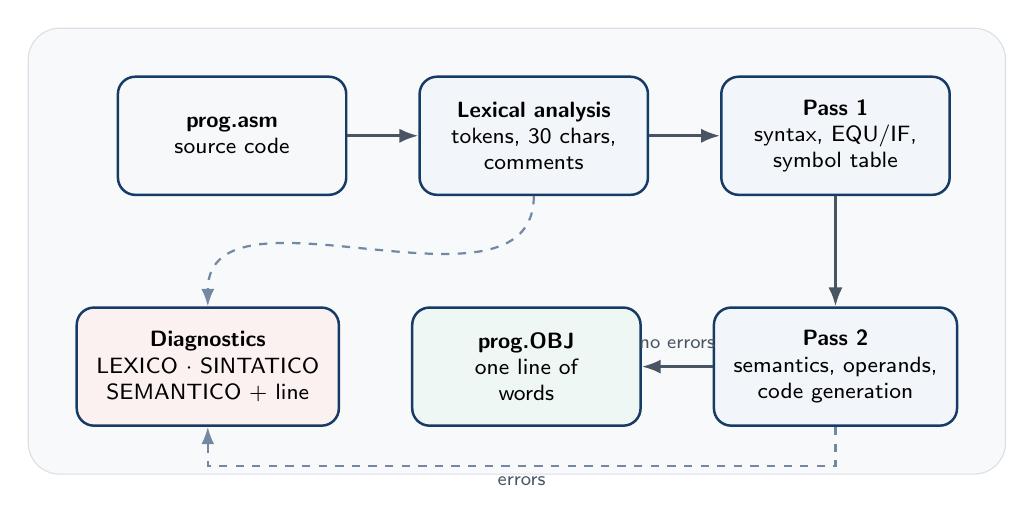
\begin{tikzpicture}[
  font=\sffamily\footnotesize, >=Latex, every node/.style={align=center},
  box/.style={rounded corners=2.2mm, draw=navy, line width=0.9pt, fill=white,
              minimum height=15mm, minimum width=29mm, inner sep=2.5mm},
  arrow/.style={-{Latex[length=2.4mm]}, line width=1pt, draw=textgray},
  warrow/.style={-{Latex[length=2.2mm]}, line width=0.8pt, draw=navy!60, dashed}
]
% row 1
\node[box, fill=grayfill] (asm) {\textbf{prog.asm}\\source code};
\node[box, right=9mm of asm, fill=bluefill] (lex) {\textbf{Lexical analysis}\\tokens, 30 chars,\\comments};
\node[box, right=9mm of lex, fill=bluefill] (p1) {\textbf{Pass 1}\\syntax, EQU/IF,\\symbol table};
% row 2
\node[box, below=14mm of p1, fill=bluefill] (p2) {\textbf{Pass 2}\\semantics, operands,\\code generation};
\node[box, left=9mm of p2, fill=greenfill] (obj) {\textbf{prog.OBJ}\\one line of\\words};
\node[box, left=9mm of obj, fill=redfill] (diag) {\textbf{Diagnostics}\\LEXICO $\cdot$ SINTATICO\\SEMANTICO + line};

\draw[arrow] (asm) -- (lex);
\draw[arrow] (lex) -- (p1);
\draw[arrow] (p1) -- (p2);
\draw[arrow] (p2) -- node[above=1mm, font=\sffamily\scriptsize, text=textgray] {no errors} (obj);
\draw[warrow] (lex.south) to[out=-90,in=90] (diag.north);
\draw[warrow] (p2.south) -- ++(0,-5mm) -| node[pos=0.25, below, font=\sffamily\scriptsize, text=textgray] {errors} (diag.south);

\begin{pgfonlayer}{background}
  \node[draw=navy!16, fill=navy!3, rounded corners=4mm, inner sep=6mm,
        fit=(asm)(lex)(p1)(p2)(obj)(diag)] {};
\end{pgfonlayer}
\end{tikzpicture}
\end{document}
